%% Version 4.3.2, 25 August 2014
%
%%%%%%%%%%%%%%%%%%%%%%%%%%%%%%%%%%%%%%%%%%%%%%%%%%%%%%%%%%%%%%%%%%%%%%
% Template.tex --  LaTeX-based template for submissions to the 
% American Meteorological Society
%
% Template developed by Amy Hendrickson, 2013, TeXnology Inc., 
% amyh@texnology.com, http://www.texnology.com
% following earlier work by Brian Papa, American Meteorological Society
%
% Email questions to latex@ametsoc.org.
%
%%%%%%%%%%%%%%%%%%%%%%%%%%%%%%%%%%%%%%%%%%%%%%%%%%%%%%%%%%%%%%%%%%%%%
% PREAMBLE
%%%%%%%%%%%%%%%%%%%%%%%%%%%%%%%%%%%%%%%%%%%%%%%%%%%%%%%%%%%%%%%%%%%%%

%% Start with one of the following:
% DOUBLE-SPACED VERSION FOR SUBMISSION TO THE AMS
\documentclass{ametsoc}

% TWO-COLUMN JOURNAL PAGE LAYOUT---FOR AUTHOR USE ONLY
% \documentclass[twocol]{ametsoc}

%%%%%%%%%%%%%%%%%%%%%%%%%%%%%%%%
%%% To be entered only if twocol option is used

\journal{jtech}

%  Please choose a journal abbreviation to use above from the following list:
% 
%   jamc     (Journal of Applied Meteorology and Climatology)
%  jtech     (Journal of Atmospheric and Oceanic Technology)
%   jhm      (Journal of Hydrometeorology)
%   jpo     (Journal of Physical Oceanography)
%   jas      (Journal of Atmospheric Sciences)	
%   jcli      (Journal of Climate)
%   mwr      (Monthly Weather Review)
%   wcas      (Weather, Climate, and Society)
%   waf       (Weather and Forecasting)
%   bams (Bulletin of the American Meteorological Society)
%   ei    (Earth Interactions)

%%%%%%%%%%%%%%%%%%%%%%%%%%%%%%%%
%Citations should be of the form ``author year''  not ``author, year''
\bibpunct{(}{)}{;}{a}{}{,}

%%%%%%%%%%%%%%%%%%%%%%%%%%%%%%%%

%%% To be entered by author:

%% May use \\ to break lines in title:

\title{Estimating $\chi$ using fast-response thermistors on traditional shipboard CTDs: sources of uncertainty and bias.}

%%% Enter authors' names, as you see in this example:
%%% Use \correspondingauthor{} and \thanks{Current Affiliation:...}
%%% immediately following the appropriate author.
%%%
%%% Note that the \correspondingauthor{} command is NECESSARY.
%%% The \thanks{} commands are OPTIONAL.

    %\authors{Author One\correspondingauthor{Author One, 
    % American Meteorological Society, 
    % 45 Beacon St., Boston, MA 02108.}
% and Author Two\thanks{Current affiliation: American Meteorological Society, 
    % 45 Beacon St., Boston, MA 02108.}}

\authors{Andy Pickering\correspondingauthor{College of Earth, Ocean, and Atmospheric Sciences, Oregon State University,Corvallis, OR.}}

%% Follow this form:
     \affiliation{College of Earth, Ocean, and Atmospheric Sciences, Oregon State University,Corvallis, OR.}

%\affiliation{}

%% Follow this form:
    %\email{latex@ametsoc.org}

\email{apickering@coas.oregonstate.edu}

%% If appropriate, add additional authors, different affiliations:
    \extraauthor{Jonathan Nash}
    \extraaffil{College of Earth, Ocean, and Atmospheric Sciences, Oregon State University,Corvallis, OR.}

    \extraauthor{James N Moum}
    \extraaffil{College of Earth, Ocean, and Atmospheric Sciences, Oregon State University,Corvallis, OR.}

    \extraauthor{Jennifer MacKinnon}
    \extraaffil{UCSD / Scripps Institute of Oceanography}



%\extraauthor{}
%\extraaffil{}

%% May repeat for a additional authors/affiliations:

%\extraauthor{}
%\extraaffil{}

%%%%%%%%%%%%%%%%%%%%%%%%%%%%%%%%%%%%%%%%%%%%%%%%%%%%%%%%%%%%%%%%%%%%%
% ABSTRACT
%
% Enter your abstract here
% Abstracts should not exceed 250 words in length!
%
% For BAMS authors only: If your article requires a Capsule Summary, please place the capsule text at the end of your abstract
% and identify it as the capsule. Example: This is the end of the abstract. (Capsule Summary) This is the capsule summary. 

\abstract{The acquisition of turbulence data from shipboard CTD profiles is attractive, as it has the potential to significantly increase the amount of deep-ocean mixing observations globally.  While data from shear-probes are easily contaminated by motion of the instrument platform, the measurement of temperature gradient is relatively insensitive to vehicle vibration, making it possible to measure temperature gradient from a shipboard CTD rosette.  The purpose of this note is to investigate the error and bias in estimating the rate of dissipation of temperature variance $\chi$ from fast thermistors mounted on traditional CTD casts.  The most significant source of error is associated with the fact that fast-response FP07 thermistors resolve only a fraction of the temperature gradient variance at the fallspeed of typical CTD casts.  Assumptions must be made about the wavenumber extent of the temperature gradient spectrum, which scales with the rate of dissipation of turbulent kinetic energy, a quantity that is not directly measured.  Here we utilize observations from a microstructure profiler with shear probes to demonstrate the validity of our method of estimating $\chi$ from thermistor data, and to assess uncertainty and bias. We then apply this methodology to temperature gradient profiles obtained from $\chi$pods mounted on a CTD (the CTD-$\chi$pod), and compare these to microstructure profiles obtained almost synoptically at the equator.  CTD-$\chi$pod estimates of $\chi$ compare favorably to the shear-probe microstructure measurements and demonstrate that the $\chi$pod method is not significantly biased.  This supports the utility of the measurement as part of the global repeat hydrography program (GO-SHIP) cruises, during which this type of data has been acquired during the past few years.}


\begin{document}

%% Necessary!
\maketitle


%%%%%%%%%%%%%%%%%%%%%%%%%%%%%%%%%%%%%%%%%%%%%%%%%%%%%%%%%%%%%%%%%%%%%
% MAIN BODY OF PAPER
%%%%%%%%%%%%%%%%%%%%%%%%%%%%%%%%%%%%%%%%%%%%%%%%%%%%%%%%%%%%%%%%%%%%%
%

%% In all cases, if there is only one entry of this type within
%% the higher level heading, use the star form: 
%%

% \section{Introduction}
% \subsection*{subsection}
% text...
% \section{Section title}

%vs

% \section{Section title}
% \subsection{subsection one}
% text...
% \subsection{subsection two}
% \section{Section title}

%%%
% \section{First primary heading}

% \subsection{First secondary heading}

% \subsubsection{First tertiary heading}

% \paragraph{First quaternary heading}


%~~~~~~~~~~~~~~~~~~~~~~
\section{Introduction}
%~~~~~~~~~~~~~~~~~~~~~~

Turbulent mixing affects the distribution of heat, salt, and nutrients throughout the global ocean. Diapycnal mixing  of cold, dense water with warmer water above maintains the abyssal overturning circulation \citep{munk66,munkwunsch98}, which affects global climate. Because the turbulence that drives mixing generally occurs at scales that are not resolved in climate models, it must be parameterized, based on either (i) aspects of the resolved model dynamics, (ii) through higher resolution models that capture the dynamics that feed energy to turbulence, or (iii) using other parameterizations that either dynamically or statistically quantify turbulent fluxes. Recent investigations have demonstrated that these models are sensitive to the magnitude and distribution of mixing \citep{meletetal13}. A comprehensive set of measurements that spans relevant dynamical regimes is needed to constrain mixing and develop more accurate parameterizations.

To quantify turbulence, typically either the dissipation rate of turbulent kinetic energy $\epsilon$ or the dissipation rate of temperature variance $\chi$ are measured. The dissipation rate of TKE may be dynamically interesting to internal wave energetics globally, since the energy flow can be tracked and then $\epsilon$ can be used to esimate the potential for mixing. The dissipation rate of temperature variance $\chi$ is one of the most easily measured direct metrics of mixing, through $K_T$. These quantities ($\epsilon$ and $\chi$) are typically computed by measuring the variance of velocity gradient or temperature gradient, which have universal theoretical forms with subranges described by power-law formulations (Figure \ref{specshapes}). The wavenumber extent and amplitude of the theoretical shear spectrum scales with $\epsilon$. In contrast, the the temperature gradient spectrum amplitude scales with both $\chi$ and $\epsilon$, and the wavenumber extent scales with $\epsilon$.

The most accurate measurements of turbulence are made with microstructure profilers equipped with shear probes.  Shear probes are used to measure the spectra of velocity shear at small enough scales that a fit to standard inertial subrange spectral shapes allows an estimate of the turbulent dissipation rate ($\epsilon$) as a fitting parameter. This technique is well-suited for targeting upper-ocean processes, but can be expensive, time-intensive, and requires considerable care and expertise. Moreover, tethered profilers can't reach abyssal depths, requiring autonomous instruments to get deeper than $\sim$1000-2000 m.  As a result, existing measurements of diapycnal mixing, especially in the deep ocean, are sparse \citep{waterhouseetal14}. In order to obtain a larger quantity of mixing estimates, considerable work has gone into inferring mixing from measurements of the outer scales of turbulence, which are easier to obtain. One popular method is the use of Thorpe scales, where diapycnal mixing is inferred from inversions in profiles of temperature or density  \citep{thorpe77,dillon82}. The size of resolvable overturn is limited by the profiling speed and instrument noise \citep{galbraithkelley96}. 
While some studies indicate relatively good agreement with microstructure and other observations, there remain questions about the general validity of the method and the assumptions made \citep{materetal15,scotti15}. Parameterizations based on profiles of shear and/or strain have also been developed and applied to estimate diapycnal mixing \citep{gregg89a,kunzeetal06,polzinetal14,whalenetal12,whalenetal15}.  However, they rely on a series of assumptions about the cascade of energy from large to small scales (they assume turbulence rates are set by an energy cascade through the internal wave field) that are often violated; numerous studies (i.e., \cite{watermanetal13}) have shown that there is significant uncertainty associated with these parameterizations, in that there can be a consistent bias in a particular region, yet the sense of the bias (i.e., over-predict vs.\ under-predict) is not known a priori. 

Quantifying turbulence from velocity shear variance (to compute the dissipation rate of turbulent kinetic energy $\epsilon$) is challenging on moorings or profiling platforms because there is usually too much vibration and/or package motion for shear-probes to be useful. Pitot-static tubes have recently been used for this purpose, plus providing independent measurements of speed \citep{moum15}. Other methods (i.e., optics or acoustics) may hold some promise, but lack of scatterers often precludes this type of measurement, especially in the abyss.  In addition, shear probes only provide $\epsilon$, not the diapycnal diffusivity of scalars, $K$, which is often inferred from $\epsilon$ by assuming a mixing efficiency $\Gamma$ \citep{osborn80} as $K=\Gamma \epsilon / N^{2}$, where $N^2$ is the buoyancy frequency.  A more direct measure of turbulent mixing is obtained from the dissipation rate of temperature variance $\chi$ \citep{osborncox72}.  This has the advantage that (i) the temperature and temperature gradient can be computed and are relatively straightforward to measure, and (ii) the estimation of mixing from $\chi$ does not require assumptions about $\Gamma$. However, the spectrum of temperature gradient extends to very small scales, so that its spectrum is seldom fully resolved (and unlike shear variance, the wavenumber extent of the temperature gradient spectrum does not scale with its amplitude, but instead depends on $\epsilon$ (Figure \ref{specshapes}). Assumptions about the spectral shape (Kraichnan vs.\ Bachelor, and the value of the ``constant'' q) and its wavenumber extent (governed by the Batchelor wavenumber $k_b=[\epsilon/(\nu D_{T}^{2})]^{1/4}$  \citep{Batchelor59}) are thus necessary to determine $\chi$ unless measurements capture the full viscous-diffusive subrange of turbulence (i.e., down to scales $\Delta x \sim 1/k_b \sim 1$mm), a criterion seldom achieved.  To resolve this, we follow \cite{alfordpinkel00b} and \cite{moumnash09} and make the assumption that $K_T=K_{\rho}$ to determine the dissipation rate as $\epsilon_{\chi}=(N^2\chi)/(2\Gamma <dT/dz>^2)$, permitting estimation of $k_b$. 


The goal of this paper is to outline and validate the methods used to compute $\chi$ and $K_T$ with $\chi$pods mounted on CTDs (Figure \ref{f1}).  We do this by applying our processing methodology to profiles of temperature gradient measured by thermistors on the `Chameleon' microstructure profiler, which provides a direct test of our methodology.  Because Chameleon is a loosely tethered profiler equipped with shear probes \citep{moumetal95}, it directly measures $\epsilon$ and allows us to test our assumptions.  Specifically, it allows us to determine biases associated with computing $\chi$ from partially-resolved temperature gradient spectra alone, as compared to computation that includes $\epsilon$, which constrains the wavenumber extent of the scalar spectra.   After establishing that the method works, we then compare CTD-$\chi$pod profiles to nearby microstructure profiles.


%~~~~~~~~~~~~~~~~~~~~~~
\section{Data }
%~~~~~~~~~~~~~~~~~~~~~~

%~~~~~~~~
\subsection{EQ14}

Data were collected on the R/V Oceanus in Fall 2014 during the EQ14 experiment to study equatorial mixing.  More than 2700 Chameleon profiles were made, along with 35 CTD-$\chi$pod profiles bracketed by Chameleon profiles in order to maintain calibrations during the cruise. Most Chameleon profiles were made to a maximum depth of about 250m, with CTD casts going to 500m or deeper. The EQ14 experiment and results are discussed in more detail in ( SJ Warner, RN Holmes, EH McHugh-Hawkins, JN Moum, 2016: Buoyant gravity currents released from tropical instability waves, JPO, in preparation) and \cite{holmesetal2016}.



%~~~~~~~~~~~~~~~~~~~~~~
\section{Methods}
%~~~~~~~~~~~~~~~~~~~~~~
%~~~~~~~~


As mentioned in the introduction, the temperature gradient spectrum is rarely fully resolved down to the small scales of turbulent mixing. The fraction of the spectrum resolved depends on the true spectrum (a function of $\chi$ and $\epsilon$), the flowspeed past the sensor ($u$), and the response of the thermistor. The GE/Thermometrics FP07 thermistors we use typically resolve frequencies up to about $f_{max}=10-15$ Hz. The maximum resolved wavenumber is then equal to $k_{max}=f_{max}/u$, while the wavenumber extent of the true spectrum varies with $k_b$ (and $\epsilon^{1/4}$). At the typical vertical fall rate of a CTD rosette ($\sim$1m/s), only about 20\% of $k_b$ is resolved at $\epsilon=10^{-10}Wkg^{-1}$ (Figure \ref{kbratVseps}). While methods have been developed to fit the observed temperature gradient spectrum to theoretical forms \citep{ruddicketal00}, these work only when a larger fraction of the temperature gradient spectrum is resolved. For the relatively high profiling speeds typical of CTD casts, we find these methods do not work well (see appendix for more details) and therefore we use the following methodology, which does not have a strongly $\epsilon$-dependent bias.

We first outline our method for estimating $\chi$, which relies on (i) determining the instantaneous flowspeed past the sensor, (ii) identifying periods where the signals may be contaminated by the wake of the CTD rosette, (iii) defining the relevant values of $N^2$ and $(dT/dz)^2$, and (iv) applying an iterative method to compute $\chi$. We then discuss some limitations and practical considerations that arise.

\subsection{Iterative Method for estimating $\chi$}

For each $\sim$1 second window, $\chi$ is estimated via the following procedure as outlined in \cite{moumnash09}. For isotropic turbulence,
\begin{equation}
\chi_T=6D_T \int_{0}^{\infty}\Psi_{T_x} (k) dk
\label{eq:chiint}
\end{equation}
where $D_T$ is the thermal diffusivity and $\Psi_{T_x} (k)$ is the wavenumber spectrum of $dT/dx$.

Note that $dT/dx$ is not actually measured; $dT/dt$ is measured, and $dT/dx$ is inferred from Taylor's frozen flow hypothesis:
 \begin{equation}
\frac{dT}{dx}=\frac{1}{u}\frac{dT}{dt}
\label{eq:2}
\end{equation}
where $u$ represents the flow speed past the sensor. The wavenumber extent of the spectrum depends on the Batchelor wavenumber $k_b$, which is related to $\epsilon$:
\begin{equation}
k_b=[\epsilon/(\nu D_{T}^{2})]^{1/4}
\label{eq:3}
\end{equation}

We assume that $K_{\rho}=K_T$ and $K_{\rho}=\Gamma \epsilon /N^2$ where the mixing efficiency $\Gamma$ is assumed to be $0.2$ \citep{moumnash09}. Then dissipation rate is computed as
\begin{equation}
\label{eq:eps}
\epsilon_{\chi}=\frac{N^2\chi_T}{2\Gamma <dT/dz>^2}
\end{equation}

Typical thermistors do not resolve the spectrum out to $k_b$, so the measured spectrum is fit to the Kraichnan form (with $q=7$) of the theoretical scalar spectrum over the range of resolved wavenumbers ($k_{min}<k<k_{max}$). The variance between the measured $[\Phi_{T_x}(k)]_{obs}$ and theoretical $[\Phi_{T_x}(k)]_{theory}$ spectra at these wavenumbers is assumed to be equal:

\begin{equation}
\int^{k_{max}}_{k_{min}}[\Phi_{T_x}(k)]_{obs}dk=\int^{k_{max}}_{k_{min}}[\Phi_{T_x}(k)]_{theory}dk
\label{eq:speceq}
\end{equation}

An iterative procedure is then used to fit and calculate $\chi$ and $\epsilon$:

\begin{enumerate}
\item First we estimate $\chi_T$ based on an initial guess of $\epsilon=10^{-7}$ $\mathrm{Wkg^{-1}}$ and compute $k_b$ via eq. \ref{eq:3}. We set $k_{max} = k_b/2$ or to a wavenumber equivalent to $f_{max}=7$ Hz [i.e., $k_{max}= 2\pi(f_{max})/u$], whichever is smaller. In general $f_{max}$ should be the highest value which is safely below the sensor's roll-off. We chose $f_{max}=7$Hz in this case based on inspection of the temperature gradient spectra and historical measurements of these sensors (see appendix for more details).
\item We then use Eq. (\ref{eq:eps}) to refine our estimate of $\epsilon$ and $k_b$ and recompute $\chi_T$ using Eqs. (\ref{eq:chiint}) and (\ref{eq:speceq}). 
\item This sequence is repeated and converges after two or three iterations.
\end{enumerate}
Note that this procedure is equivalent to the explicit formulation of \citep{alfordpinkel00b}, except we use the Kraichnan theoretical form instead of the Batchelor spectrum for $[\Phi_{T_x}(k)]_{theory}$. At wavenumbers below the spectral peak, there is little distinction between the Kraichnan and Batchelor spectra, so this factor does not affect the computational bias.

\subsection{CTD-$\chi$pod Data Processing}

We next review the basic outline for processing each CTD-$\chi$pod profile. The moored $\chi$pod instrument \citep{moumnash09} has a pressure sensor, compass, and pitot-static tube. In contrast, the CTD-$\chi$pod requires pressure measured by the CTD and has no independent speed measurement other that $dp/dt$ from the CTD.
\begin{enumerate}
\item The correct time-offset for the $\chi$pod clock is determined by aligning highpass-filtered $dp/dt$ from the 24Hz CTD data to  integrated vertical accelerations measured by the $\chi$pod. $\chi$pod clock drift is small, typically on the order of 1 sec/week, but it is imperative to get records aligned within $< 0.5$ s so that the correct value of $u$ is used. In the case of the CTD-$\chi$pod we assume $u$ is solely due to the vertical motion of the CTD cage, i.e. $u=dp/dt$.
\item Low-order polynomial calibration coefficients are determined to convert thermistor voltages from $\chi$pod to ITS90 temperature (as measured by
the CTD). Figure \ref{f2} shows an example of the aligned and calibrated CTD-$\chi$pod timeseries for one cast. Note the significant differences in amount of variance associated with the two sensors during down and up casts. For the upward-mounted sensor (T1), the downcast signal is largely associated with the CTD wake, as is the upcast for the downward-mounted sensor (T2). Only the `clean' portions of the cast (e.g., the T1 upcast and the T2 downcast) are used in the $\chi$pod calculations.
\item Depth loops are identified and flagged in the 24Hz CTD data (Figure \ref{depthloops2}). $\chi$pod data during these times are discarded since the signals are likely contaminated by the wake of the CTD. We use a vertical velocity threshold of $0.3$m/s and throw out data within 2m of the identified loops. Even for profiles that are significantly affected by ship heaving, good segments of data are obtained over a majority of the depths after removing contaminated data, allowing us to compute values in nearly every 10m bin. 
\item Buoyancy frequency $N^2$ and temperature gradient $dT/dz$ are computed from 1-m binned CTD data, and averaged over a scale of 10m. The results are not very sensitive to the averaging interval (see appendix for more details).
\item Half-overlapping 1 sec windows of data are used to estimate $\chi$ following the methods described in \cite{moumnash09}, as outlined in the previous section.
\end{enumerate}


%%~~~~~~
\subsection{Example Spectra and Fits}

Examples of the observed (from FP07 thermistor on Chameleon) and fit spectra are shown in Figure \ref{specexamp}, for two windows where a low and high dissipation rate was observed. The Chameleon spectra (magenta) shown is the theoretical Kraichnan spectra for the values of $\chi$ and $\epsilon$ estimated using the shear-probe data. The $\chi$pod fit is the estimate from applying the $\chi$pod method to just the thermistor data for the same window. Note that at lower $\epsilon$, a larger fraction of $k_b$ is observed and the peak of the spectrum is almost resolved. At higher $\epsilon$, less of the spectrum is resolved and the spectral peak is well above the maximum resolved wavenumber. Even so, the iterative $\chi$pod method gives an accurate estimate of $\chi$. The $\chi$pod and Chameleon fits are performed over the same wavenumber range and thus match there. However, the higher-wavenumber portions of the fit spectra differ since the Chameleon fits use the observed $k_b$ to determine the wavenumber extent.


%~~~~~~~~~~
%\subsection{flowspeed past the sensor}

%The flowspeed past the thermistor is needed to convert the measured temperature derivative $dT/dt$ to a spatial gradient. For the CTD-$\chi$pod, the largest contribution to the flowspeed is usually the vertical velocity of the CTD package ($dp/dt$), which is close to 1m/s on average, so we typically neglect the horizontal component of velocity in converting from frequency to wavenumber spectra. Although usually a good approximation, errors may be introduced where horizontal velocities are large. Note that because it is the total instantaneous velocity magnitude that represents flow past the sensor, neglecting the horizontal component of velocity (assuming $u=dp/dt$) means we underestimate the true flowspeed past the sensor. When the CTD package is equipped with LADCP, the true flowspeed can be measured. In some cases where the CTD was not equipped with LADCP, it would seem that the ship's ADCP could be used to estimate the horizontal component of velocity. However, because the CTD does not travel perfectly vertically in strong currents, this is difficult to do in practice. In a strong horizontal flow, the CTD will drift with the current while descending, lowering the flow relative to the sensors. On the upcasts, the CTD will be pulled against the current, increasing the flow relative to the sensors. %Since the CTD in EQ14 was not equipped with LADCP, we use $dp/dt$ as the flowspeed, and estimate potential errors in the appendix.



%~~~~~~~~~~~~~~~~~~~~~~
\section{Results }
%~~~~~~~~~~~~~~~~~~~~~~


\subsection{Direct Test of $\chi$pod Method}

We begin by utilizing the highly-resolved data from the freely-falling turbulence profiler, Chameleon (for which both $\epsilon$ and $\chi$ are measured) to test the assumptions in our method of estimating $\chi$. We first apply the $\chi$pod method to each Chameleon profile, using only the FP07 thermistor data. These results, which we refer to as $\chi_{\chi}^{cham}$ and assume no independent knowledge of $\epsilon$, are then compared to $\chi_{\epsilon}^{cham}$, computed by integrating the theoretical temperature gradient spectrum where $k_b$ is computed directly from shear-probe derived $\epsilon$. Qualitatively, $\chi_{\chi}^{cham}$ and $\chi_{\epsilon}^{cham}$ show very similar depth and time patterns (Figure \ref{eq14_eps_pcolor}) and appear to agree in magnitude. A more quantitative comparison (Figure \ref{eq14_chi_2dhist}), shows the two are well-correlated over five orders of magnitude. The distribution of $log_{10}$ of the $\chi$ ratios is approximately normal, with a mean of $\mu=-0.1$ and standard deviation of $\sigma=0.51$. This indicates a low bias of $\chi_{\chi}^{cham}$ relative to $\chi_{\epsilon}^{cham}$ of 20\% and random variation of a factor of 3. The magnitude of the bias increases slightly at higher values of $\epsilon_{cham}$ (Table \ref{t1}), reaching a low bias of approximately 40$\%$ for $-6<log_{10}[\epsilon_{cham}]<-5$. The cause of this bias is unknown, but may be related to the spectrum shifting to higher wavenumbers at larger $\epsilon$. 



%~~~~~~~~~~~~~~~~~~~~~~
\subsection{ CTD$\chi$pod - Chameleon Comparison}
%~~~~~~~~~~~~~~~~~~~~~~

Having demonstrated that the method works using Chameleon data, we now compare $\chi_{\chi}^{ctd}$ from CTD-mounted $\chi$pods to $\chi_{\epsilon}^{cham}$. In contrast to the Chameleon data, the CTD is more strongly coupled to the ship, and therefore subject to more vibration, heaving, and artificial turbulence created by the rosette. A total of 35 CTD-$\chi$pod casts were performed, bracketed with Chameleon profiles immediately before and after. We first compare CTD-$\chi$pod profiles to the mean of the two Chameleon profiles bracketing each cast, both averaged in 5m depth bins (Figure \ref{eq14_cdtChi_vs_cham}). The two are correlated, with considerable scatter. A histogram of the log of ratios is approximately normal and has a mean of $-0.31$, indicating a small negative bias. Since we expect significant natural variability in turbulence even between adjacent Chameleon profiles, we investigate further to determine if the observed $\chi$pod variability is of a similar magnitude or greater than expected. Scatter plots of before vs. after Chameleon profiles (not shown), typically separated by about an hour, show a similar level of scatter as the differences between methods, suggesting that the observed differences (Figure \ref{eq14_cdtChi_vs_cham}) can be explained by natural variability in turbulence. This is further demonstrated by histograms of the ratio of $\chi$ from adjacent casts (Figure \ref{eq14_cdtChi_vs_cham_hist}) which show that the variability between CTD $\chi$pod and Chameleon casts is similar to the natural variability between before/after Chameleon profiles. Profiles from all CTD-Chameleon pairs averaged in time and 40m depth bins (Figure \ref{ctd_cham_chi_boot_all}) overlap within 95\% confidence limits at all depths where there exists good data for both. Averages of subsets of these profiles that were clustered in position/time (not shown) also agree well. We conclude that the variability between CTD$\chi$pod and Chameleon profiles is indistinguishable from natural variability in turbulence levels.


%~~~~~~~~~~~~~~~~~~~~~~
\section{Discussion}
%~~~~~~~~~~~~~~~~~~~~~~

We have shown that $\chi$ can be accurately estimated from $\chi$pods attached to CTD rosettes. The method also estimates $K_T$ and $\epsilon$, but we have left discussion of these for a future paper since they involve more assumptions and uncertainties. One major assumption is the mixing efficiency $\Gamma$. A value of $0.2$ is commonly assumed, but evidence suggests this may vary significantly. \cite{moumnash09} found a bias in $\chi$ of up to 1.6 for $\Gamma$ values ranging from $0.1$ to $0.35$.  Another major assumption in the $\chi$pod method is that $K_T=K_{\rho}$ \citep{moum96b}. 

The goal of CTD-$\chi$pods is to expand the number and spatial coverage of ocean mixing observations. The census of \cite{waterhouseetal14} found less than 20 locations where full-depth microstructure profiles were taken (see their figure 1c), all of which had less than 100 profiles. We have already deployed CTD $\chi$pods during several process experiments and on several GO-SHIP repeat-hydrography cruises, obtaining more than 1700 full-depth profiles of $\chi$ over a wide range of locations. We plan to continue regular deployment on GO-SHIP and similar cruises, adding $\chi$ to the suite of variables regularly measured. The expanding database of mixing measurements from CTD-$\chi$pods will also enable testing of other commonly-used or new mixing parameterizations. This has the potential to be transformative for the field, allowing the community to develop and test global turbulence parameterizations, use estimates of turbulence along with the CLIVAR repeat hydrography data for inverse models and water mass modification calculations, identify hotspots of turbulence to target with future process experiments, and compare with in-situ chemical and biological measurements made routinely on repeat hydrography cruises.

% thanks Jen for some of above text!

%~~~~~~~~~~~~~~~~~~~~~~
\section{Conclusions}
%~~~~~~~~~~~~~~~~~~~~~~

\begin{itemize}
\item The $\chi$pod method for estimating $\chi$ was directly applied to temperature gradients measured by the Chameleon microstructure profiler on $>$ 2700 profiles during the EQ14 cruise. The estimated $\chi_{\chi}$ agrees well with $\chi_{\epsilon}$ calculated using $\epsilon$ from shear probes over a wide range of magnitudes (Figure \ref{eq14_chi_2dhist}) with little or no bias, demonstrating that the method works.
\item CTD-$\chi$pod profiles were also compared to nearby Chameleon profiles during the cruise. Variability between CTD-$\chi$pod and Chameleon estimates of $\chi$ is indistinguishable from natural variability between Chameleon profiles. Time-averaged profiles of $\chi$ from both platforms agree within 95\% confidence limits, and no significant bias was detected between the estimates of $\chi$.
\item We conclude that estimates of $\chi$ made from the CTD-$\chi$pod platform are robust and reliable.
\end{itemize}



%%%%%%%%%%%%%%%%%%%%%%%%%%%%%%%%%%%%%%%%%%%%%%%%%%%%%%%%%%%%%%%%%%%%%
% ACKNOWLEDGMENTS
%%%%%%%%%%%%%%%%%%%%%%%%%%%%%%%%%%%%%%%%%%%%%%%%%%%%%%%%%%%%%%%%%%%%%
%
\acknowledgments
The EQ14 experiment was funded by budget (NSF?) 1256620. We thank the Captain and crew of R/V Oceanus. Pavan Vutukur, Craig Van Appledorn, Mike Neeley-Brown made the sensors. Aurelie Moulin, Ryan Holmes, Sally Warner and Anna Savage helped to collect the data.

%%%%%%%%%%%%%%%%%%%%%%%%%%%%%%%%%%%%%%%%%%%%%%%%%%%%%%%%%%%%%%%%%%%%%
% APPENDIXES
%%%%%%%%%%%%%%%%%%%%%%%%%%%%%%%%%%%%%%%%%%%%%%%%%%%%%%%%%%%%%%%%%%%%%
%
% Use \appendix if there is only one appendix.
%\appendix

% Use \appendix[A], \appendix}[B], if you have multiple appendixes.
%\appendix[A]

%% Appendix title is necessary! For appendix title:

\appendix[A]

%% Appendix title is necessary! For appendix title:
\appendixtitle{Sensitivity Analysis}

\section{Flowspeed Past Sensor}

To quantify the potential error in the CTD-$\chi$pod calculations from ignoring horizontal velocities and assuming the flow speed is equal to the vertical speed of the CTD rosette, we repeated the calculations with constant offsets added to the flowspeed. Note that since the total magnitude of velocity is used, $dp/dt$ is a minimum estimate of the true speed. Adding $0.1$($1$)m/s results in a mean percent error of -14(-58) percent (Figure \ref{FspdSensHist}), small compared the large natural variability in turbulence and uncertainty in our measurements. Note that increasing the velocity tends to result in smaller values of $\chi$, since it shifts the spectrum to lower wavenumbers. 

We also looked for any systematic biases associated with flowpseed. We found that $\chi$ was biased high for very small speeds ($u<25$cm/s). This could be associated with contamination by CTD wake or entrained water when the CTD slows.  These values were discarded for our analysis.

%When the CTD package is equipped with LADCP, the true flowspeed can be measured. In some cases where the CTD was not equipped with LADCP, it would seem that the ship's ADCP could be used to estimate the horizontal component of velocity. However, because the CTD does not travel perfectly vertically in strong currents, this is difficult to do in practice. In a strong horizontal flow, the CTD will drift with the current while descending, lowering the flow relative to the sensors. On the upcasts, the CTD will be pulled against the current, increasing the flow relative to the sensors.
%\appendix[B]

%\clearpage
%~~~~~~~~~~~~~~~~~~~~~~~~~

%
%\section{$N^2$ and $dT/dz$}
%
%We investigated the sensitivity of the calculations to the scale over which $N^2$, $dT/dz$ are averaged. The iterative method to estimate chi requires the background stratification $N^2$ and temperature gradient $dT/dz$. The estimate of $\chi$ is insensitive to these scales. However, dissipation rate $\epsilon$ and diffusivity $K_T$ are more strongly affected because they are linearly related to these values. Computing $N^2$ and $dT/dz$ over smaller scales (less than a few m) results in larger values and hence some larger values of $K_T$.


\appendix[B]

%% Appendix title is necessary! For appendix title:
\appendixtitle{Test of MLE fitting method}

We also tested the spectrum fitting method of \cite{ruddicketal00} and compared to our $\chi$pod method. The MLE method works well and gives similar results to our method at true $\epsilon$ values less than about $10^{-9}$, but severely underestimates $\chi$ at larger values of epsilon, where only a small fraction of the spectrum is resolved (Figure \ref{mlefits}). At lower profiling speeds we would expect the MLE method to work better, as more of the spectrum will be resolved for a given value of $\epsilon$.


\appendix[C]


% PlotVarCapt_DiffXfr.m

%% Appendix title is necessary! For appendix title:
\appendixtitle{Thermistor Frequency Response}
Prior to 2009, the transfer function for each FP07 thermistor was measured by profiling adjacent to a thermocouple in Yaquina Bay, OR. However, measuring the transfer function for each individual thermistor proved too expensive and time-consuming, and since that time a generic transfer function has been used. Figure \ref{xfr} shows the measured transfer functions for 2008. The majority of the transfer functions are similar for frequencies up to about 10 Hz, and begin to significantly differ above that. To estimate the potential error in not using a transfer function, we calculated the $\%$ of spectral variance captured for each of the measured functions. For frequencies up to 7Hz, more than 95\% is captured for 88\% of the measured functions. If frequencies up to 15hz are used, more than 95 \% variance is captured only 67\% of the time. Using only frequencies up to 7Hz (where the transfer function is equal to or very close to unity) avoids the issue of the unknown transfer functions.



%%% Appendix section numbering (note, skip \section and begin with \subsection)
% \subsection{First primary heading}

% \subsubsection{First secondary heading}

% \paragraph{First tertiary heading}

%% Important!
%\appendcaption{<appendix letter and number>}{<caption>} 
%must be used for figures and tables in appendixes, e.g.,
%
%\begin{figure}
%\noindent\includegraphics[width=19pc,angle=0]{figure01.pdf}\\
%\appendcaption{A1}{Caption here.}
%\end{figure}
%
% All appendix figures/tables should be placed in order AFTER the main figures/tables, i.e., tables, appendix tables, figures, appendix figures.
%
%%%%%%%%%%%%%%%%%%%%%%%%%%%%%%%%%%%%%%%%%%%%%%%%%%%%%%%%%%%%%%%%%%%%%
% REFERENCES
%%%%%%%%%%%%%%%%%%%%%%%%%%%%%%%%%%%%%%%%%%%%%%%%%%%%%%%%%%%%%%%%%%%%%
% Make your BibTeX bibliography by using these commands:
 \bibliographystyle{ametsoc2014}
 \bibliography{main.bib}


%%%%%%%%%%%%%%%%%%%%%%%%%%%%%%%%%%%%%%%%%%%%%%%%%%%%%%%%%%%%%%%%%%%%%
% TABLES
%%%%%%%%%%%%%%%%%%%%%%%%%%%%%%%%%%%%%%%%%%%%%%%%%%%%%%%%%%%%%%%%%%%%%
%% Enter tables at the end of the document, before figures.
%%
%
%\begin{table}[t]
%\caption{This is a sample table caption and table layout.  Enter as many tables as
%  necessary at the end of your manuscript. Table from Lorenz (1963).}\label{t1}
%\begin{center}
%\begin{tabular}{ccccrrcrc}
%\hline\hline
%$N$ & $X$ & $Y$ & $Z$\\
%\hline
% 0000 & 0000 & 0010 & 0000 \\
% 0005 & 0004 & 0012 & 0000 \\
% 0010 & 0009 & 0020 & 0000 \\
% 0015 & 0016 & 0036 & 0002 \\
% 0020 & 0030 & 0066 & 0007 \\
% 0025 & 0054 & 0115 & 0024 \\
%\hline
%\end{tabular}
%\end{center}
%\end{table}


% MakeBiasTable.m
\begin{table}[t]
\caption{Biases and stand. dev. of ratios of $log_{10} [\chi_{\chi}/\chi_{\epsilon}]$ for different ranges of $\epsilon_{cham}$.}\label{t1}
\begin{center}
\begin{tabular}{|c|c|c|}
\hline\hline
$\epsilon_{cham}$ range & bias & sd \\ 
\hline
$-9 < \epsilon < -8$ & -0.04 & 0.47 \\ 
\hline
$-8 < \epsilon < -7$ & -0.15 & 0.51 \\ 
\hline
$-7 < \epsilon < -6$ & -0.18 & 0.54 \\ 
\hline
$-6 < \epsilon < -5$ & -0.2 & 0.55 \\ 
\hline
\hline\hline
\end{tabular}
\end{center}
\end{table}


%%%%%%%%%%%%%%%%%%%%%%%%%%%%%%%%%%%%%%%%%%%%%%%%%%%%%%%%%%%%%%%%%%%%%
% FIGURES
%%%%%%%%%%%%%%%%%%%%%%%%%%%%%%%%%%%%%%%%%%%%%%%%%%%%%%%%%%%%%%%%%%%%%
%% Enter figures at the end of the document, after tables.
%%
%
%\begin{figure}[t]
%  \noindent\includegraphics[width=19pc,angle=0]{figure01.pdf}\\
%  \caption{Enter the caption for your figure here.  Repeat as
%  necessary for each of your figures. Figure from \protect\cite{Knutti2008}.}\label{f1}
%\end{figure}

\graphicspath{
{/Users/Andy/Cruises_Research/ChiPod/ChiPod_Methods_Paper/figures/}
}

\begin{figure}[t]
  \noindent\includegraphics[width=38pc,angle=0]{SpecShapes.png}\\
  \caption{Top: Theoretical (Nasmyth) wavenumber spectra for velocity shear, for two different values of $\epsilon$. Lower: Theoretical (Kraichnan) wavenumber spectra for temperature gradient, for two different values of $\epsilon$ and $\chi$. Note the amplitudes of temperature gradient spectra depend on both $\epsilon$ and $\chi$, while the shear spectra depend only on $\epsilon$. Diamonds indicate the Batchelor wavenumber for each, which depends only on $\epsilon$. Vertical dashed lines indicate range of wavenumbers used for $\chi$pod fit assuming $u=1$m/s.}
  \label{specshapes}
\end{figure}


\begin{figure}[t]
  \noindent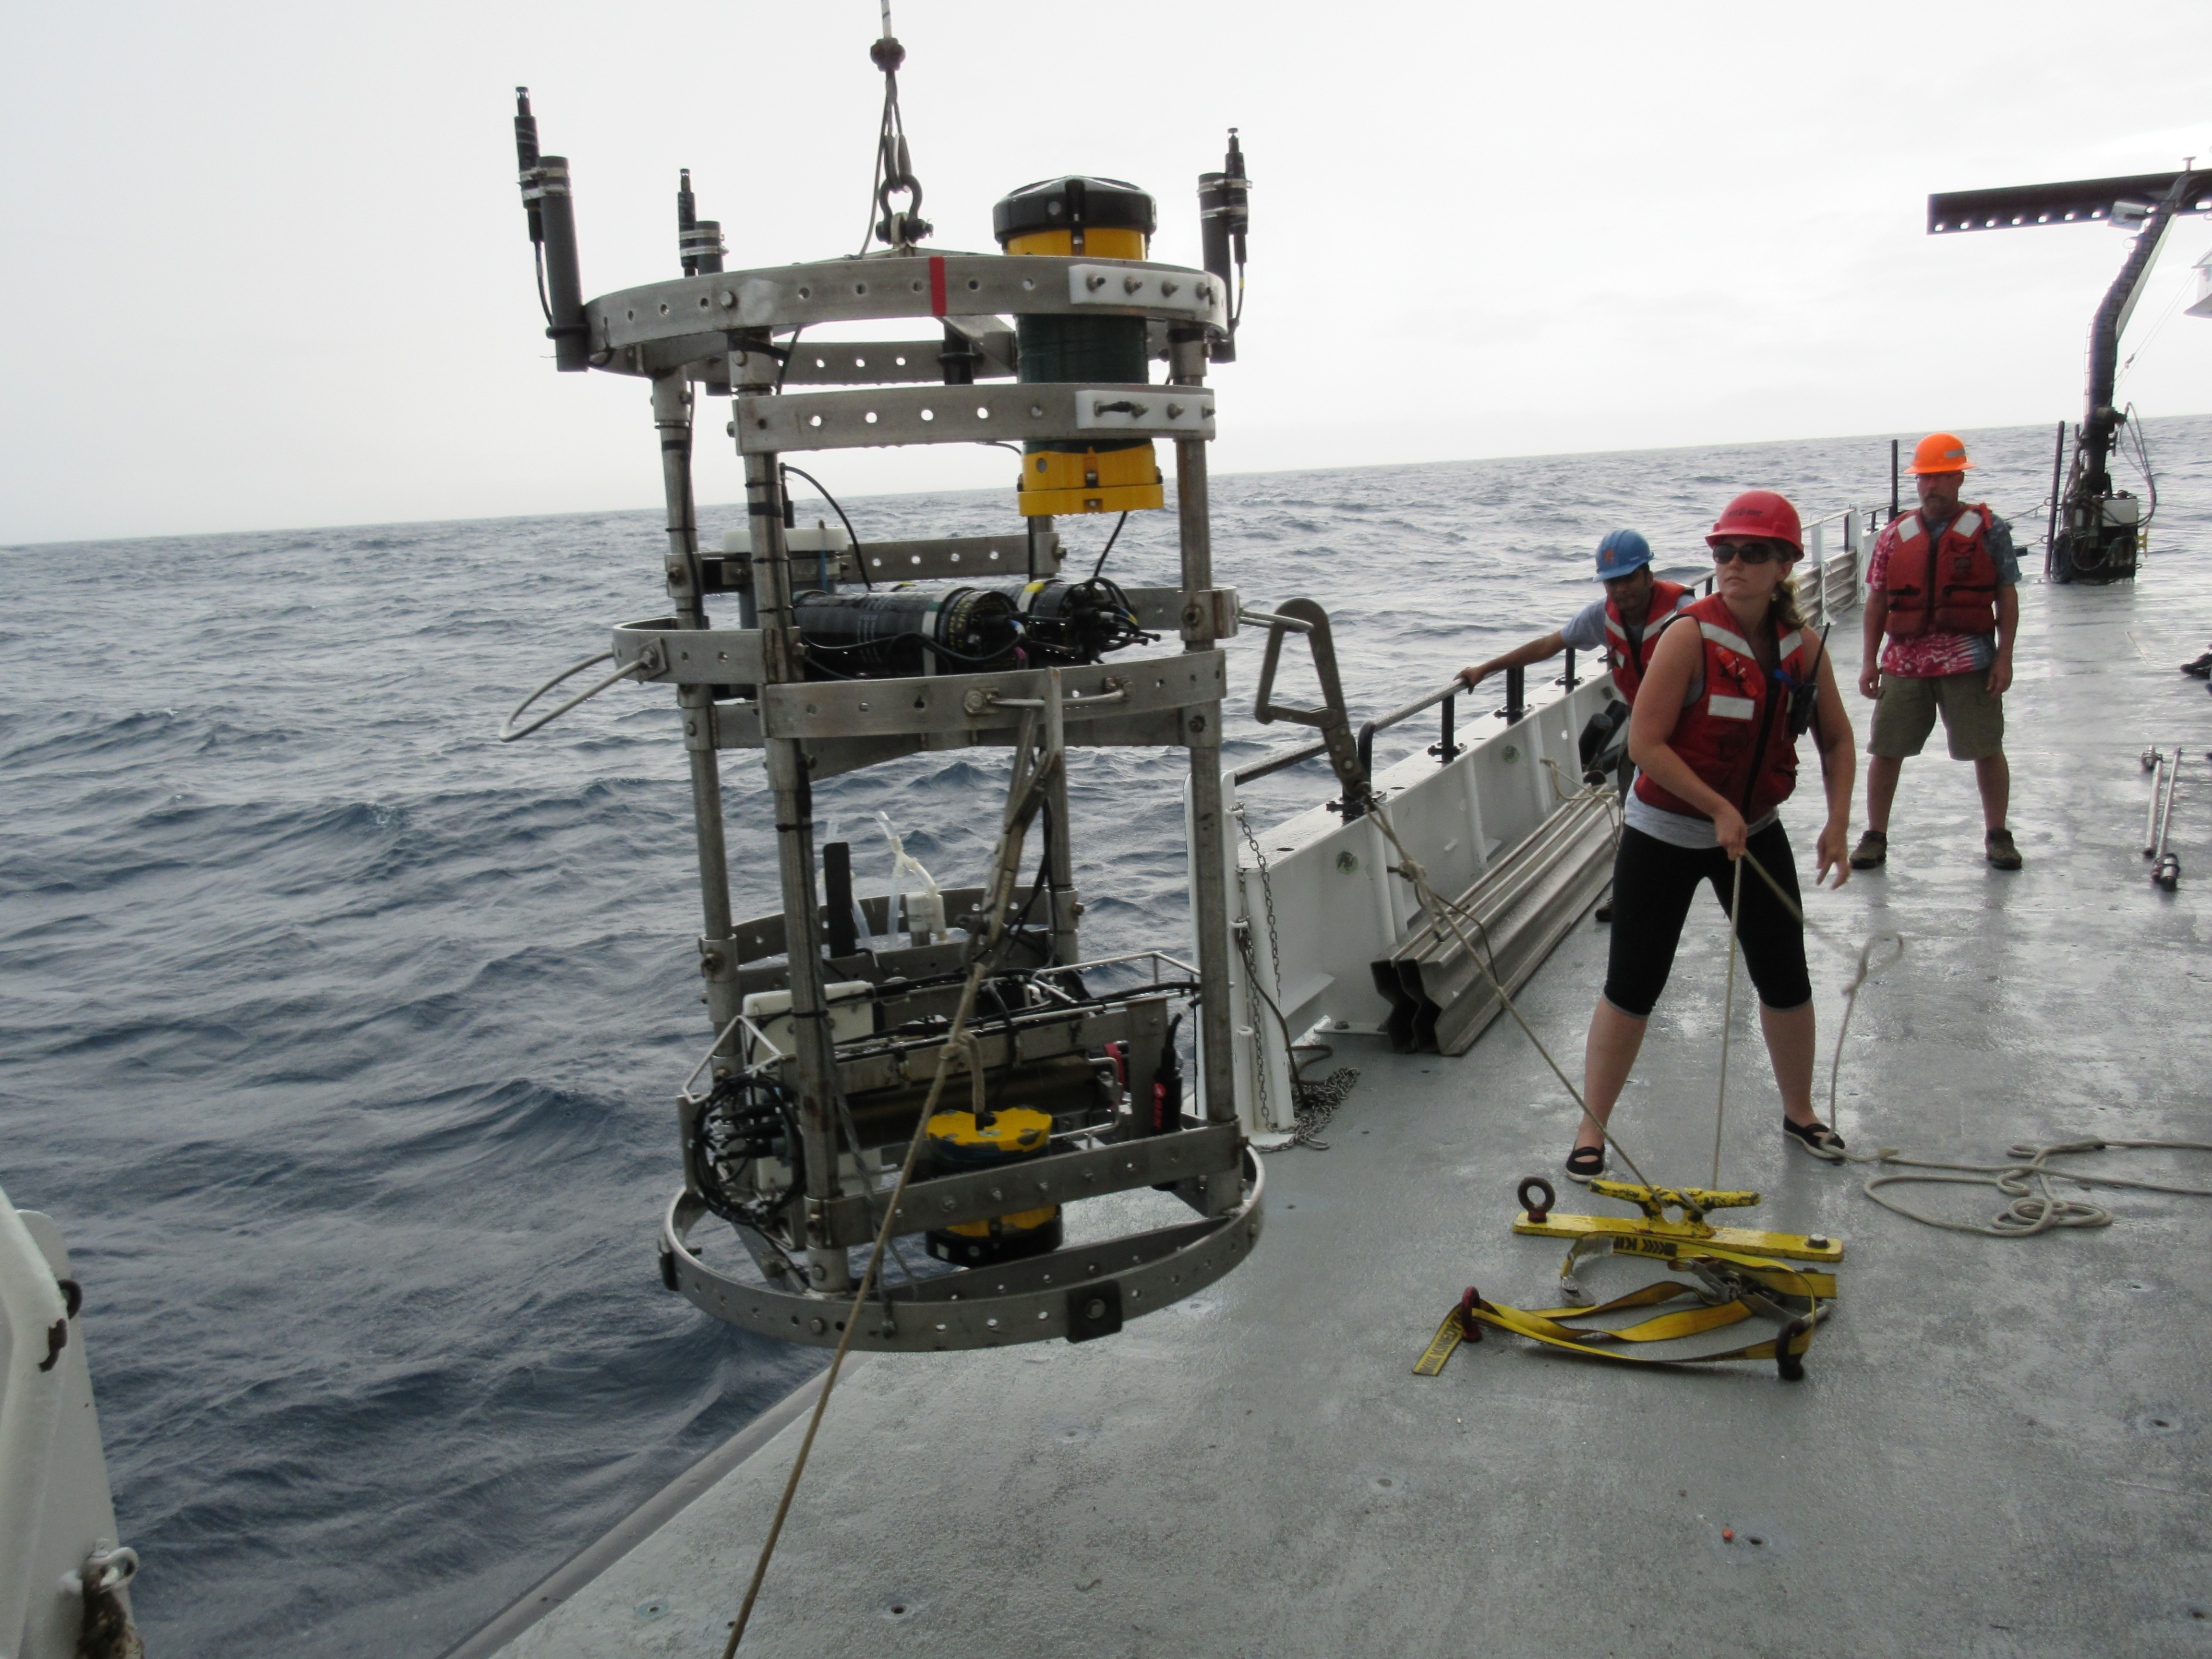
\includegraphics[width=38pc,angle=0]{IMG_0198.JPG}\\
  \caption{Photo of CTD rosette during EQ14 with $\chi$pods attached.}
  \label{f1}
\end{figure}


\begin{figure}[t]
  \noindent\includegraphics[width=38pc,angle=0]{kbratVsEps.png}\\
  \caption{Ratio of the maximum observed wavenumber $k_{max}=f_{max}/u$ to the Batchelor wavenumber $k_b$ for different values of $\epsilon$, assuming a $f_{max}=7Hz$. Each line is for a different flowspeed.}
  \label{kbratVseps}
\end{figure}

%% PlotDepthLoops.m
%\begin{figure}[t]
%  \noindent\includegraphics[width=38pc,angle=0]{DepthLoopExample.png}\\
%  \caption{Left: Raw CTD pressure for one cast, with data flagged as depth-loops in red. Right: Histogram of the number of good 1 sec windows in each 10m bin, after removing contaminated data.}
%  \label{depthloops}
%\end{figure}


% PlotExampleTS.m
\begin{figure}[t]
  \noindent\includegraphics[width=38pc,angle=0]{SN1001_Cast02_Fig5_T_P_dTdz_fspd.png}\\
  \caption{Example timeseries from one CTD cast during EQ14. a) CTD pressure. b) Fallspeed of CTD ($dp/dt$) .c) Vertical and horizontal accelerations measured by $\chi$pod. d) Temperature from CTD and (calibrated) $\chi$pod sensors. T2 is offset slightly for visualization. e) Temperature derivative $dT/dt$ measured by the upward-looking $\chi$pod sensor T1. f) Temperature derivative $dT/dt$ measured by the downward-looking $\chi$pod sensor T2.}
  \label{f2}
\end{figure}

\begin{figure}[t]
  \noindent\includegraphics[width=38pc,angle=0]{DepthLoopExample2TS.png}\\
  \caption{Portion of a CTD cast showing depth vs time (top) during an upcast, with data flagged as loops in red. Lower panel shows corresponding $\chi$pod timeseries of $dT/dt$ for that time with discarded loop data in red. Note that variance tends to be larger during depth loops due to entrained water and CTD-induced turbulence.}
  \label{depthloops2}
\end{figure}


\begin{figure}[t]
  \noindent\includegraphics[width=38pc,angle=0]{ExSpec_HiLowEps.png}\\
  \caption{Two example temperature gradient spectra from an EQ14 Chameleon profile, for high (top) and low (bottom) values of $\epsilon$. Solid black lines with circles show the observed temperature-gradient spectra from the thermistor on Chameleon. Dashed black line shows the fitted theoretical Kraichnan spectra estimated by applying the $\chi$pod method to the thermistor data only. Magenta line is Kraichnan spectra for Chameleon $\chi$ and $\epsilon$ measured at the same depth, using the shear probe data as well. Vertical dashed blue(red) lines indicate the minimum (maximum) wavenumber used in the $\chi$pod calculation. The Batchelor wavenumber $k_b$ is also indicated by the vertical magenta line.}
  \label{specexamp}
\end{figure}


% Plot_chiProc_vs_actual_EQ14
\begin{figure}[t]
  \noindent\includegraphics[width=38pc,angle=0]{EQ14_chiVsTrue_chi_zsm10m_fmax7Hz_respcorr0_fc_99hz_gamma20.png}\\
  \caption{Depth-time plots of $log_{10}\chi$ from both methods for EQ14 data. Top: $\chi$pod method using only FP07 data from Chameleon. Black diamonds indicate casts used for comparison with CTD-$\chi$pod profiles. Bottom: Chameleon measurements using FP07 and shear probe data.}
  \label{eq14_eps_pcolor}
\end{figure}


\begin{figure}[t]
  \noindent\includegraphics[width=38pc,angle=0]{EQ14_2dhist_chi_WITHhist_zsm10m_fmax7Hz_respcorr0_fc_99hz_gamma20.png}\\
  \caption{Top: 2D histogram of $log_{10}(\chi)$ from Chameleon (x-axis) and $\chi$pod method (y-axes). Values from each profile were averaged in the same 5m depth bins. Bottom: Normalized histogram of $\log_{10}[\chi_{\chi}^{cham}/\chi_{\epsilon}^{cham}]$. Vertical dashed line indicates the mean of the the distribution.}
  \label{eq14_chi_2dhist}
\end{figure}


%Scatter_CTDchiVsCham_Pairs.m
\begin{figure}[t]
  \noindent\includegraphics[width=38pc,angle=0]{EQ14_ctdChipod_vs_chamMean_chi_scatter_WITHhist.png}\\
  \caption{Left: Scatter plot of $\chi$ from CTD-$\chi$pod profiles versus the mean of bracketing Chameleon profiles. Black dashed line shows 1:1, red are $\pm$ 10 X. Right: Normalized histogram of the log of ratios.}
  \label{eq14_cdtChi_vs_cham}
\end{figure}

%Make_Combined_Cham_for_CTD_pairs.m
% PlotHistChiRatio_CTDchamPairs.m
\begin{figure}[t]
  \noindent\includegraphics[width=38pc,angle=0]{EQ14_CtdChipod_hist_chi_ratios.png}\\
  \caption{Histogram of $log_{10}$ of the ratio of $\chi$ for nearby casts. The first set is for the before ($\chi_{\epsilon1}^{cham}$) and after ($\chi_{\epsilon2}^{cham}$ Chameleon profiles. The 2nd is CTD-$\chi$pod profiles ($\chi_{\chi}^{ctd}$) versus the before($\chi_{\epsilon1}^{cham}$) profiles. The last is CTD-$\chi$pod profiles ($\chi_{\chi}^{ctd}$) versus the after($\chi_{\epsilon2}^{cham}$) profiles. Dashed lines show the medians of each set.  Note that bias is small/zero, and the variability (spread) between CTD/cham is similar to the natural variability between cham profiles.}
  \label{eq14_cdtChi_vs_cham_hist}
\end{figure}

% Plot_Pairs_MeanProfile.m
\begin{figure}[t]
  \noindent\includegraphics[width=38pc,angle=0]{EQ14_chi_cham_meanProf_all.png}\\
  \caption{Time mean of $\chi$ for all CTD-$\chi$pod - Chameleon cast pairs, with 95\% bootstrap confidence intervals.}
  \label{ctd_cham_chi_boot_all}
\end{figure}

\begin{figure}[t]
  \noindent\includegraphics[width=38pc,angle=0]{Hist_perr_fspdvary.png}\\
  \caption{Histogram of \% error for $\chi$ computed with constant added to fallspeed, in order to examine sensitivity to fallspeed. Vertical lines indicate the mean of each distribution.}
  \label{FspdSensHist}
\end{figure}

\begin{figure}[t]
  \noindent\includegraphics[width=38pc,angle=0]{MLEfitsEQ14_Whist.png}\\
  \caption{Left: 2D histograms of $\chi$ computed using the iterative $\chi$pod method (top) and the MLE fit (bottom) versus $\chi$ computed from Chameleon. Note that the MLE method underestimates $\chi$ at larger magnitudes. Right: Histograms of the log of ratios for different ranges of $\epsilon$. The mean of each distribution is given above.}
  \label{mlefits}
\end{figure}


\begin{figure}[t]
  \noindent\includegraphics[width=38pc,angle=0]{yq08a_TransFunc.png}\\
  \caption{Measured FP07 thermistor transfer functions from historical database. Vertical dashed lines show the frequency range used in $\chi$pod method. Dashed blue line is a generic transfer function found to best match measured functions.}
  \label{xfr}
\end{figure}



\end{document}